\documentclass{article}[11pt]
%Required: You must have these
\usepackage{graphicx}
\usepackage{tabularx}
\usepackage{natbib}

\usepackage{array}
\usepackage{amsmath}
%\usepackage[backend=bibtex]{biblatex}
\setkeys{Gin}{width=0.8\textwidth}
%\setlength{\captionmargin}{30pt}
\setlength{\abovecaptionskip}{10pt}
\setlength{\belowcaptionskip}{10pt}
\topmargin -1.5cm 
\oddsidemargin -0.04cm 
\evensidemargin -0.04cm 
\textwidth 16.59cm
\textheight 23.94cm 
\parskip 7.2pt 
\renewcommand{\baselinestretch}{1.2} 	
\parindent 0pt

\bibliographystyle{..//..//refs/styles/besjournals.bst}
\usepackage{xr-hyper}
%\usepackage{hyperref}
\usepackage{lineo}
\linenumbers
\title{Flower-leaf phenological sequence variation in the American Plums (\textit{Prunus} sect. \textit{Prunocerasus}) reflects adaption to aridity}

\usepackage{Sweave}
\begin{document}
\input{outline-concordance}
\maketitle


\section*{Introduction}
%<<label=numbers, echo=FALSE, results=hide, message=FALSE>>=
%rm(list=ls()) 
%options(stringsAsFactors = FALSE)
%require(brms,quietly = TRUE)
%setwd("~/Documents/git/proterant/investment/Input")
%load("pcerasus.Rda")
%doyeff<-round(fixef(mod.ord.scale.phlyo)[6],digits=2)
%doyints<-round(fixef(mod.ord.scale.phlyo)[6,3:4],digits=3)


\noindent Woody perennials have a unique ability among plants to seasonally begin reproduction prior to vegetative growth. This flowering-first phenological sequence known as hysteranthy, proteranthy or precocious flowering is particularly common in temperate forests around the globe \citep{Rathcke_1985}. A number of studies suggest that this flower-leaf sequences (FLSs) are under selection, and that hysteranthy has functional significance \citep{Gougherty2018,Buonaiuto2020,Guo2014}.

\noindent The most common, and well-tested explanation for the evolution of hysteranthy in temperate forests is that it is adaptive for wind-pollination, as leafless canopies increase wind speeds for pollen transport and reduce the likelihood of pollen interception on vegetation \citep{Whitehead1969,Niklas1985}. However, this hypothesis fails to address the prevalence of hysteranthous taxa that are biotically-pollinated. Approximately 30\% of woody plant species of Eastern temperate forests of North America flower before leafing out, and of these, approximately 20\% are biotically pollinated  \citep{Buonaiuto2020}. Despite the pervasiveness of this phenological syndrome, direct tests of the function of hysteranthy in biotically pollinated taxa are rare for temperate forest species.

Yet looking to other biomes in which hysteranthous flowering is also common offers important insights regarding the function of hysteranthy in temperate, biotically-pollinated taxa. In the dry-deciduous tropics of South and Central America, flowering during the leafless period is also common \citep{Rathcke_1985,Franklin2016}. In these ecosystems, flowering is associated with a recovery in plant water status due to leaf drop \citep{Borchert1983,Reich1984}. By temporally separating leaf and flower activity, woody plants can partition the hydraulic demand across the season, alleviating water stress \citep{Gougherty2018,Franklin2016}. These physiological observations suggest that hysteranthous flowering may be an adaptation to arid environments.

It is unclear whether this hydraulic demand hypothesis (also known as water dynamic hypothesis \citep{Gougherty2018} or water limitation hypothesis \citep{Buonaiuto2020}) is relevant in the temperate zone where forests are rarely water-limited in the early season during which flowering and leafing occur \citep{Polgar2011}.%, and evidence of links between hysteranthy and aridity tolerance is mixed \citep{Gougherty2018,Buonaiuto2020} 
Yet the hypothesis yields several predictions that can be tested to evaluate whether hysteranthy serves to increase aridity tolerance in temperate flora:
\begin{enumerate}
\item Hysteranthous taxa should be found in dryer habitats compared to closely related, non-hysteranthous species.
\item Hysteranthy may be linked to other reproductive traits associated with dry environments such as reduced flower and fruit size \citep{Herrera:2009aa,Liu:2013ua}.
%\item Additionally, flower-leaf sequences can be highly variable within individuals across time \citep{Buonaiuto2020}, and if hysteranthy contributes to aridity tolerance, climate variability may be positively correlated with variability in hysteranthy.
\end{enumerate}
\noindent With mounting evidence anthropogenic climate change is both driving shifts in flower-leaf sequences \citep{Ma2020:aa} and changing geographic patterns of water availability \citep{Overpeck11856}, understanding the functional significance of hysteranthy is vital to forecasting the demography and performance of forest communities in an era of global climate change. However, there are two major methodological challenges to testing the hydraulic demand hypothesis:

\noindent First, characteristics like aridity tolerance, are the emergent product of a suite of biological traits \citep{Simova:2017vk}. Thus, when analyzing selective drivers of any particular trait at large taxonomic scales, unmeasured trait differences may obscure the estimated effects of the trait of interest, biasing results. This is a common problem in trait-based ecology, and one of the most promising solutions for understanding the functional significance of hysteranthy in woody plants is through character deconstruction \citep{Terribile2009}; comparing flower-leaf sequences variation for only a subset of taxa of shared phylogenetic and morphological character.   

\noindent A second challenge for robust testing of hysteranthy hypotheses is that most characterizations of flower-leaf phenological sequences are based on expert-opinion verbal descriptions (e.g. ``flowers before leaves" or ``flower before/with leaves"), which make comparisons across taxa, time and space difficult and sensitive to observer bias  \citep[see;][]{Buonaiuto2020}. 

\noindent This problem can be overcome by adopting standardized quantitative measures of plant phenology for observational studies and applying them to historic data records. Herbarium records are an excellent source of data that can be leveraged for quantitative phenological measurements \citep{Willis2017}, but have not be used widely to investigate variability of flower-leaf sequences variation among and within species.

\noindent In this study,we used herbaria records to to quantify flower-leaf sequences both within and among species in the American plums, (subspecies  \textit{prunus}, sect. \textit{prunocerasus}. We then evaluated the association between hysteranthy and several ecological and morphological traits to test the predictions of the hydraulic demand hypothesis of hysteranthy. Our findings both clarify the hypothesized function of flower-leaf sequence variation in biotically-pollinated taxa, and offer insights into how flower-leaf sequences may impact species distributions as climate continues to change.


%<<>>=
%mich.data<-read.csv("..//..//sub_projs/MTSV_USFS/michdata_final.csv")
%table(mich.data$pro2,mich.data$Pollination)

%table(mich.data$pro)
%42/147
%table(mich.data$pro2)
%82/147



\section*{Methods}
\subsection{Study system}
\noindent The genus \texit{Prunus} comprises approximately 200 species distributed across the globe \citep{Chin:2014wu}, Within the genus, The American plums (\textit{Prunus} subspp. \textit{prunus} sect. \textit{prunocerasus}) offer potential for a higher resolution investigation of drivers of hysteranthous flowering. The 16 species that make up the section are distributed across North America and, like the genus \textit{Prunus} at large, show pronounced inter-specific variation in flower-leaf sequences. While within the larger genus species can be separated into three distinct morphological clades by inflorescence architecture (solitary, corymbose or racemose) all members of the section share solitary inflorescences \citep{Shaw:2004aa} allowing for  refined character deconstruction. Species in this section are well represented in herbaria records (Fig. \ref{fig:mappy}), making them a tractable group to measure and assess variation in flower-leaf sequences as well as other ecological and morphological characteristics related to the hydraulic demand hypothesis. 

\subsection{Quantifying flower-leaf sequence variation}
We obtained digital herbarium specimens for all member of the section \textit{Prunocerasus} from the Consortium of Midwest Herbaria Database. To quantify the flower-leaf sequence sequence variation within and across species we randomly sample 200 specimens for each species and scored the phenological development of flower and leaves in accordance with using a modified BBCH scale for woody plants \citep{Finn2007}. In total, we evaluated the phenology of 2521 specimens, but only specimens with visible flower were included in this analysis (n=1009). We reconstructed the phylogenetic relationships among species in this group based on the tree topology in \citet{Shaw:2004aa}. Following the methods of \citet{Granfen1989} we computed branch lengths for this phylogeny by assigning each node a height and computing the distance between upper and lower nodes using the R package ``ape" \citep{}.

To quantify FLS variation, we fit an ordinal, hierarchical, Bayesian, phylogenetic mixed model \citep{Garamszegi2014} to assess the likelihood an individual would be at any given vegetative BBCH phase while flowering. Because we expect that hysteranthy is more likely to occur earlier in the flowering period and species differ in their flowering periods, we included the day of the observation as a varying slope, main covariate effect in the model and species and phylogeny as random effects. The model is written below:\\

$logit(P(Y \leq j)) &= \beta_{[j]sp[i]}+ \beta_{[j]sp[i]}+ \beta_{day of year[sp[i]]}*X_1+ \epsilon_{i}$\\
  
   \epsilon_i & \sim N(0,\sigma^2_y) \\ 
   
   where Y is the ordinal outcome (leaf stage) and j is the number of categories (1,2,...6). $P(Y \leq j))$ is the probability of Y less than of equal to a category j&=1,...j&-1.  In this varying slope and intercept model, $\beta_{[j]}$ describes an intercept for each category [1,2,...6], while slope \$beta_{day of year[sp[i]]}$ is constant across categories. 
  
  \noindent The influence of the phylogeny $\alpha_{phylo}$ was modeled as follows:\\
  \alpha_{sp} & \sim N(\mu_{\alpha}, COR[\sigma^2_{phylo}]) \\
  
  \noindent THe $\alpha$ for species effects independent of the phylogeny was modeled as follows:\\
  \alpha_{sp} & \sim N(\mu_{\alpha}, \sigma^2_{species}) \\

 We fit the model in the R package ``brms" \citep{Burkner2018} using weakly informative priors, and ran the model on four chains with a warmup of 3,000 iterations and 4,000 sampling iterations for a total of 4,000 sampling iterations. Model fit was assessed with Rhats <1.01 and high effective sample sizes and no divergent transitions.
 
Because the day of observation strongly influenced the BBCH stage likelihood, quantifying flower-leaf sequences among species was intractable without accounting for this temporal trend. To address this issues, we used our model to predict the likelihood each species would be observed at a given vegetative BBCH stage during flowering at the 0\%, 25\% 50\% and 75\% quartiles of their flowering period. We then developed a flower-leaf sequence index, by assigning a numerical score to each species per seasonal quantile, and summing over the full flowering season. In each seasonal quantile, species received a 1 if more that 50\% of their probability distribution occurred at BBCH 0 and BBCH 09 and a 0 if not. These values were summed across the season generating an index from 0 (never hysteranthous) to 4 (hysteranthous through late season (Q75)), where 1&= hysteranthous at start of season, 2&= hysteranthous through early season  (Q25) and 3 &= hysteranthous  through mid season (Q50). We also used two alternative indexing schemes ($>$25\% of the probability distribution occured at BBCH 0 and $>$40\% of the probability distribution occurred at BBCH 0 and BBCH 09). 

\subsection{Evaluating the hydralic demand hypothesis}

To test the predictions of the hydralic demand hypothesis of hysteranthy we obtained data on petal length, fruit diameter and directly from herbarium specimens and characterized the aridity of the sites specimens were collected from using the Palmer Modified Drought Index (PDSI).

\noindent For our morphological measurements, we sampled an additional 321 specimens measured the petal length of up to 10 randomly selected petals per specimen (n=2757) using ImageJ image processing software. We also used ImageJ to measure the diameter of fruits on an additional 316 specimens, measuring up to 5 fruit per specimen (n=224).
We computed the average Palmer Modified Drought Index score from 1900-2017 for every \textit{Prunocerasus} specimen in the database (n=2305) from the North America Drought Atlas \citep{Cook2004}.

We than used Bayesian phylogenetic mixed models to test the relationship between flower-leaf sequence index scores and each of the variables. In these models, we included species and phylogeny as the random effect. For our PDSI model, we did not include phylogeny as a random effect as PDSI is a environmental trait rather than a biological one. \textit{Question for Jonathan: Does this check out?}

The model structure is written below: 

  y_i &= \alpha_{ind/sp[i]} +\alpha_{phylo[i]} + \beta_{hyst.index}*X_{hyst.index} + \epsilon_i\\
  
  \epsilon_i & \sim N(0,\sigma^2_y) \\ %Check this
  
  \noindent The effect of the phylogeny was model as above.% and here, the individual effects within species were modeled:\\
  %alpha_{ind/sp} & \sim N(\mu_{\alpha}, \sigma^2_{ind/sp}) \\
  
Like above, we fit these models in the R package ``brms" \citep{Burkner2018} using weakly informative priors, and ran the model on four chains with a warmup of 3,500 iterations and 4,500 sampling iterations for a total of 4,000 sampling iterations. Model fit was assessed with Rhats <1.01 and high effective sample sizes and no divergent transitions. We also ran each model using our two alternative FLS indexing approaches to make sure our particular indexing approach was not influencing our results (see Suppliment for details).

%\noindent Because our data dependent and independent were collect we employed a sequential modeling approach to first estimate the mean and standard error of the posterior distribution of trait values for each species then model the relationship between these estimate and the likelihood of hysteranthy using Bayesian measurement error models. This approach propagates the error in the initial estimates of trait values into the our final model, yielding a more accurate evaluation than using mean trait values alone \citep{}. For each parameter of interest, we ran Bayesian phylogenetic mixed-effects models with our measured traits as the response variable and species as the random effect. For traits like flower petal length and fruit diameters than included multiple measurements per specimen, we included specimen ID as an additional random effect. The model structure is written below:

%\noindent Then using each of these trait mean estimates as predictors, we modeled their associations with flower leaf sequences OF using a repeat measure phylogenetic mixed ordinal regression in brms \citep{}. Because we found the three predictors of interested to be highly colinear (pariwise correlations >0.5), we ran one regression model per predictor trait to avoid skewing our model inference due to multi-collinearity \citep{MacElreath, Nations}.

%For all models in the sequences,


\section*{Results}
\subsection*{Quantifying flower leaf sequences in the American plums}
We found substantial inter-specific differences in flower-leaf sequences within the American plums, and that patterns were strongly dependent on the day of observations, with observations later in the the flowering season of each species decreasing the likely hood of finding flowers open during early vegetative BBCH phases ($\beta_{doy}$ 0.03, $CI_{50}$ [0.02,0.03] ). Based on our flower leaf sequence index, two species (\textit{P. umbellata},\text{P. mexicana}) were likely to be hysteranthous regardless of the time of observation and three species (\textit{P. rivularis},\texit{P. subcordata}, and \textit{P. texana}) were always most likely to flower after level expansion began (Fig. \ref{fig:phylo2}). All other species displayed intermediate phenotypes with five species mostly likely to hysteranthous at the start of the season (\textit{P. alleghaniensis},\texit{P. americana},\textit{P. hortulana},\textit{P. munsoniana} and \texit{P. nigra}), one species through early season (\textit{P gracilis}) and two species through mid season (\textit{P. angustifolia}, \textit{P. maritima}) (Fig \ref{fig:phylo2}). %% check this based on the figure

\subsection*{Evaluating the Hydraulic demand hypothesis}
We found a negative association between flower-leaf sequence index and mean pdsi ($\beta$: -0.03 ,$CI_{50}$[-0.05,  0.02] ,Fig. \ref{fig:prunes}a.), suggesting that species that displayed hysteranthous flowering later into their flowering season were found in dryer locations. 

We found a negative association between flower-leaf sequence index and both  petal length and fruit diameter (-.21, $CI_{50}$"[-0.38 -0.04],-1.40, $CI_{50}$[-1.97 -0.82] respectively), though the relationship between FLS index and fruit size was much stronger (Fig. \ref{fig:prunes}b.,c.).

\section*{Discussion}

\subsection*{Aridity tolerance and flower-leaf sequence variation}

Our analyses suggest that within the American plums, hysteranthous taxa occur in more arid environments and are associated with drought-tolerant reproductive traits like reduced flower and fruit size. These associations support the hydraulic demand hypothesis of hysteranthous flowering. These results suggest that even though water limitation less common during the flowering season in temperate trees, the temporal segregation of flowering and leaf phenology can still impact whole plant water status later in the season.

Studies that have compared the transpiration rates among flowers and leaves that occur together provide insights to the potential importance of this seasonal partitioning for maintaining water status. These studies report floral transpiration rates can range from 20\%-60\% of leaves under comparable conditions \citep{Whiley:1988uf,Roddy:2012wn} which can drive loss of stomatal conductance and low photosythetic rates \citep{Galen:1999vr}. A recent study \citet{Liu:2017wg} comparing hydraulic properties of flowers and leaves in two hysteranthous Magnolias, found that sap flow to flowers was 22-55\% that of leaves. When considering species in or study specifically, the xylem conductivity of spring floral branches of  \textit{Prunus americana} is reported to be ~20\% of summer foliage branches \citep{McMann:2022ww}.Together these magnitudes of water loss through flowers suggested support our hypothesis (say better).

The relationship between flower and fruit size and hysteranthy needs some thinking about. It is well established that larger flowers demand more resources to maintain turgor and reproductive function \citep{Galen:1999vr,Lambrecht:2007ur}. Therefore a classic ecological tradeoff might predict hysteranthy compensates for larger flowers and fruits in dry environments. The fact that we found the opposite suggest rather, that these drought adaptations might be part of a suite of traits that operate to increase the aridity tolerance of a species.

Of course, selection on both phenology and floral traits is driven by a number of other factors than just plant hydraulics. The support we found for the hydraic demand hypothesis does not rule out other eco-evo drivers shaping the flower-leaf sequences of insect-pollinated. In fact, the relationship we observed bwetween hysteranthy with flowering and fruit size could also be evidence to alternative hypotheses for FLS.

\subsection*{Alternative hypotheses of flower-leaf sequence variation in biotically-pollinated woody plants}
The negative relationship between hysteranthy and flower size we observed in our analyses reflects a tradeoff predicted by the insect visibility hypthothesis of hysteranthous flower. This hypothesis suggests that flow


\bibliography{..//..//..//sub_projs/refs/hyst_outline.bib} 




\newpage
\section*{Figures}
    \begin{figure}[h!]
    \centering
 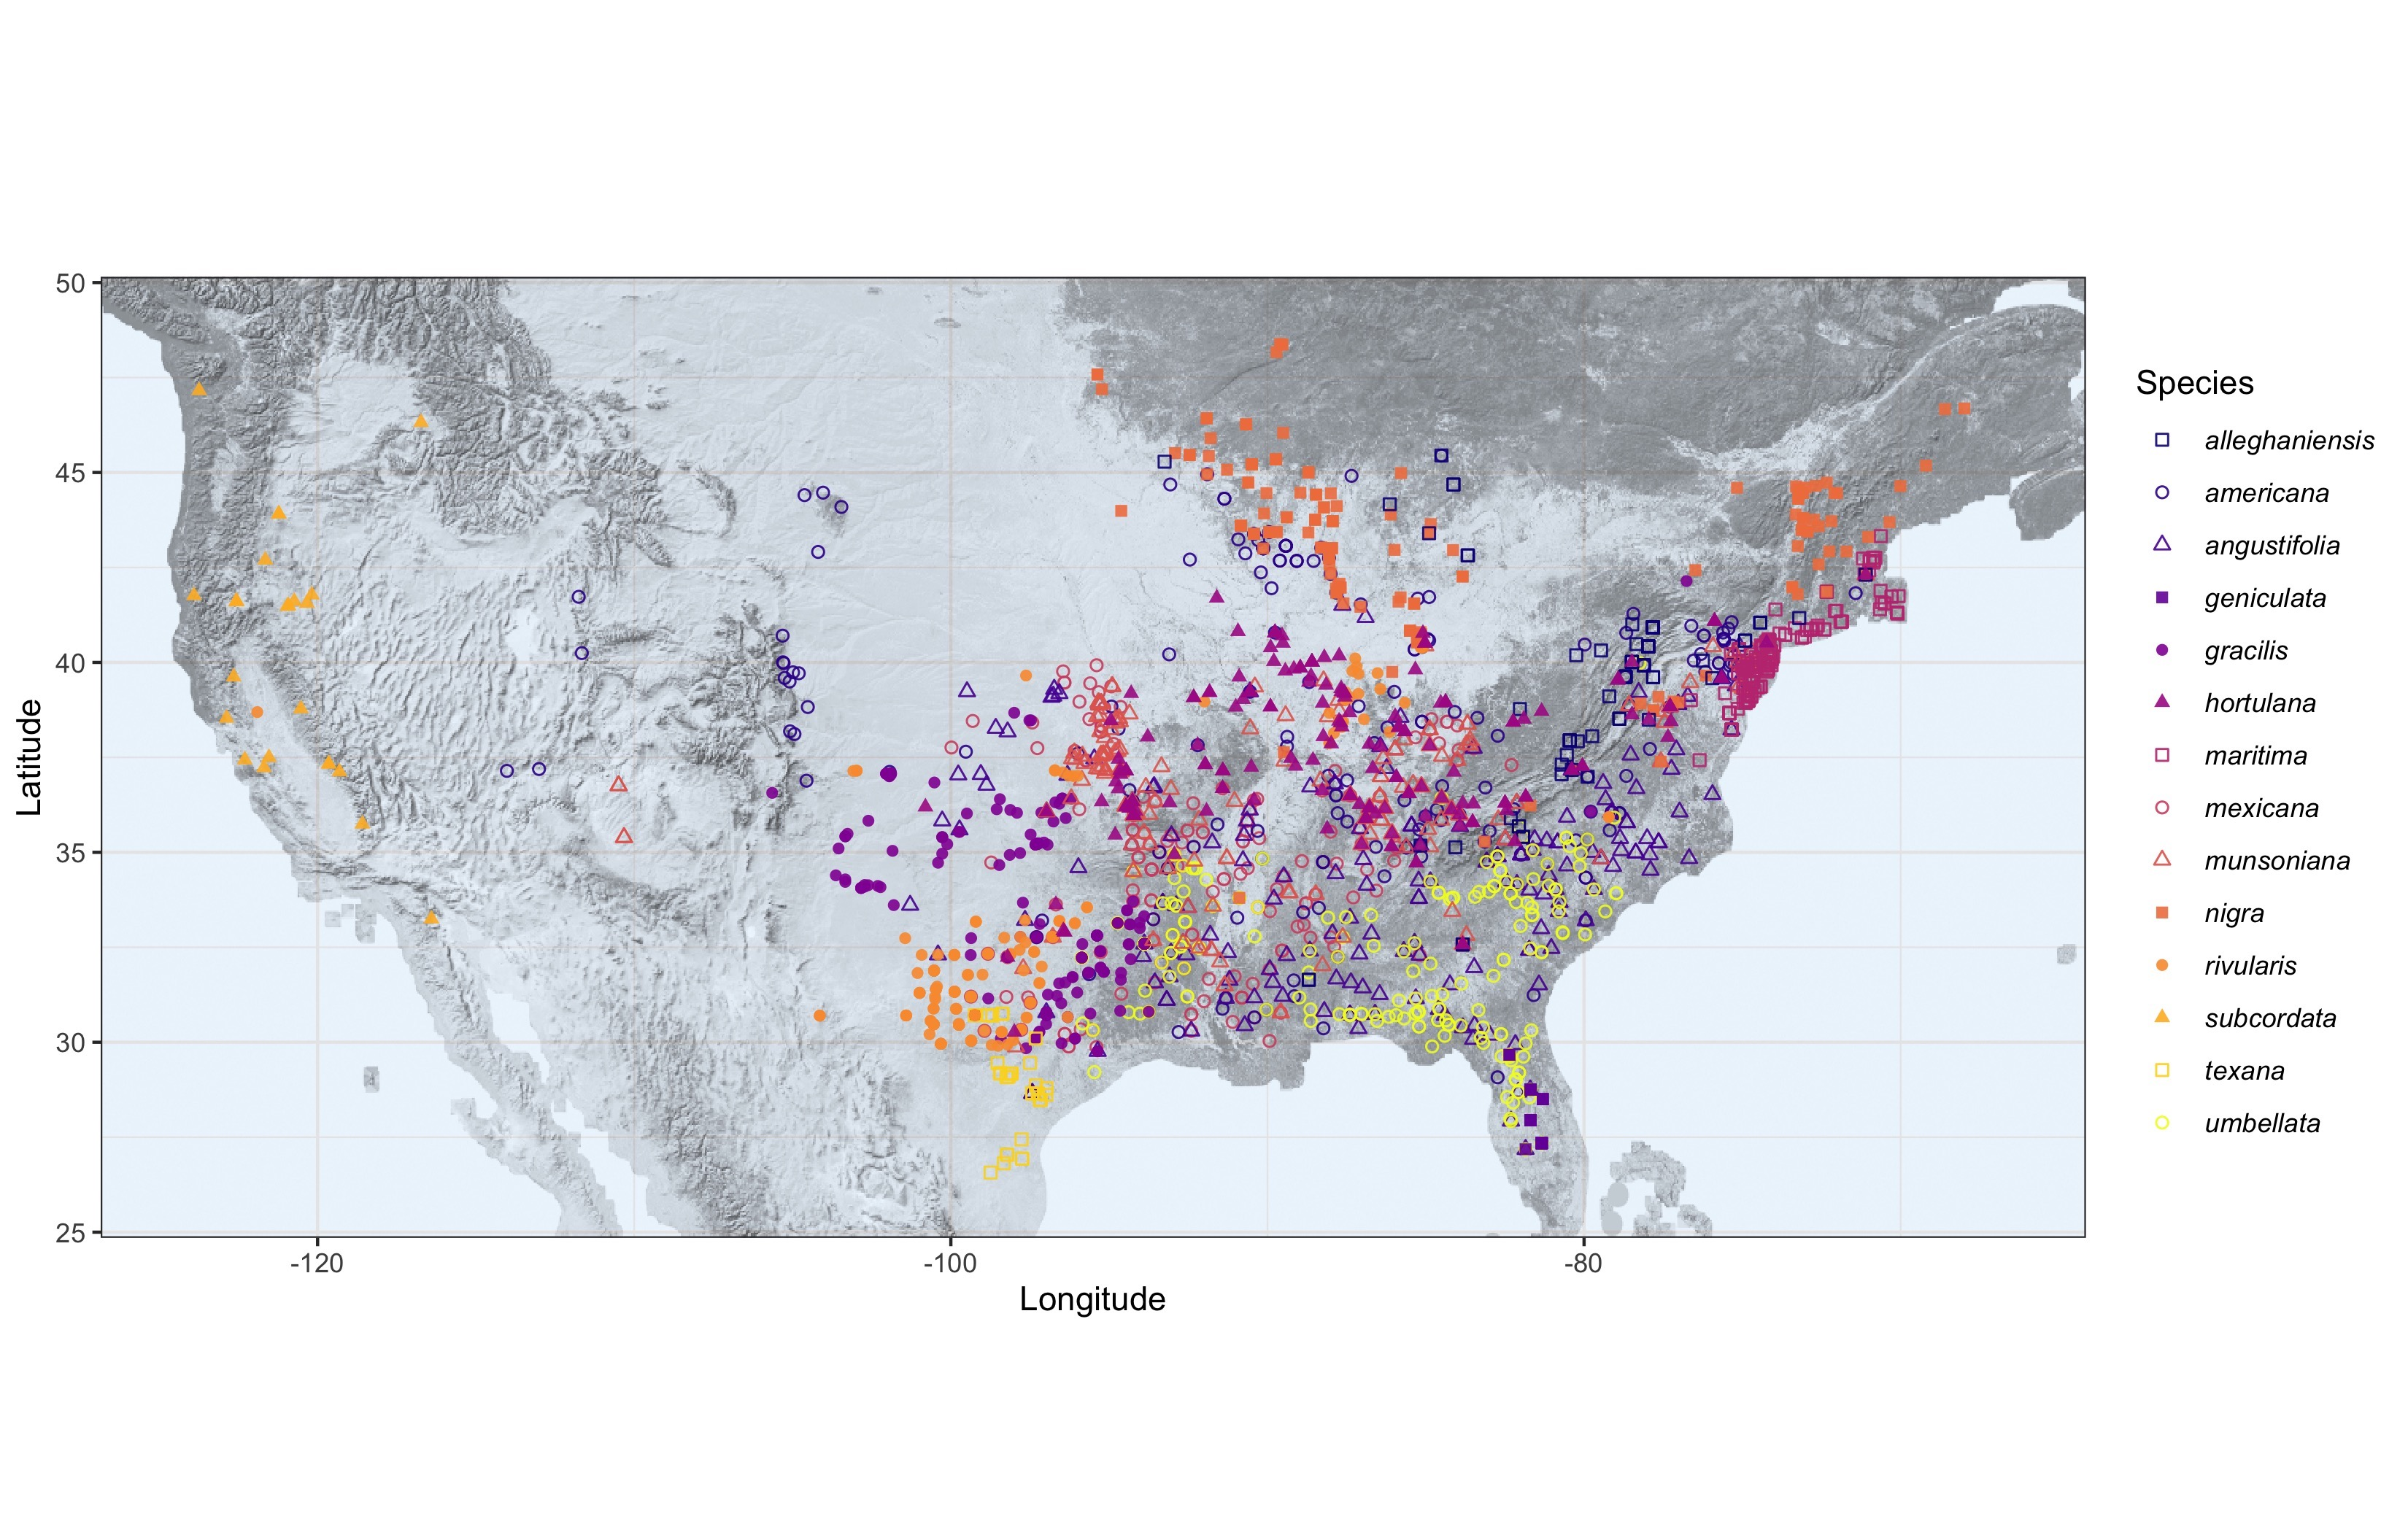
\includegraphics[width=\textwidth]{..//..//Plots/Prunus-Map-raster-plasma.jpeg}
    \caption{}
    \label{fig:mappy}
\end{figure}



\begin{figure}[h!]
    \centering
 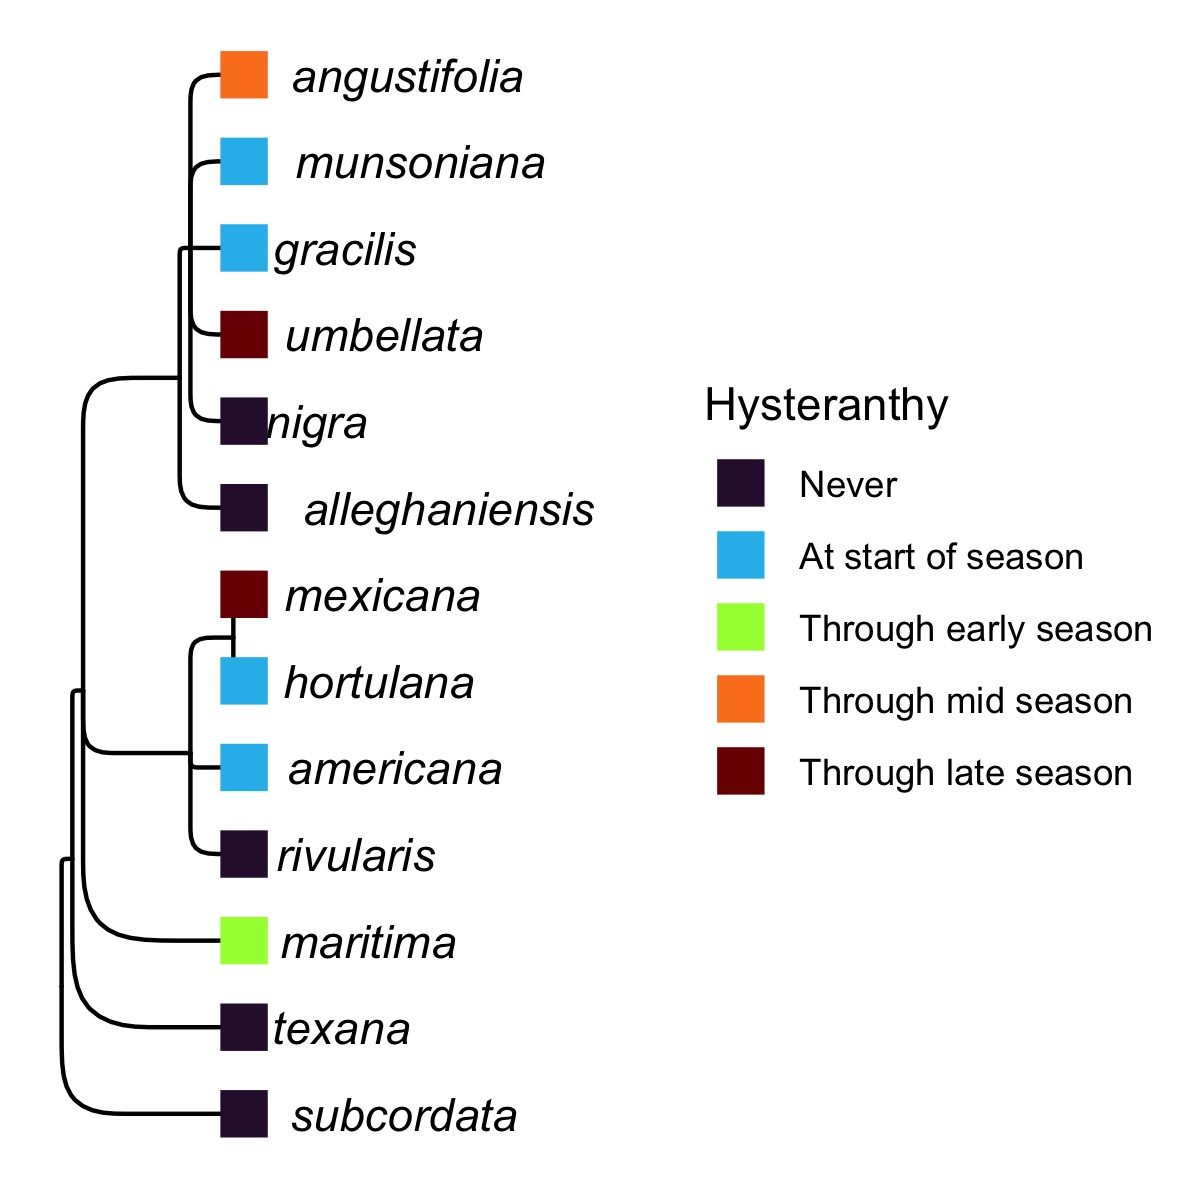
\includegraphics[width=.6\textwidth]{..//..//Plots/phylosig2.jpeg}
    \caption{}
    \label{fig:phylo2}
\end{figure}


\begin{figure}[h!]
    \centering
 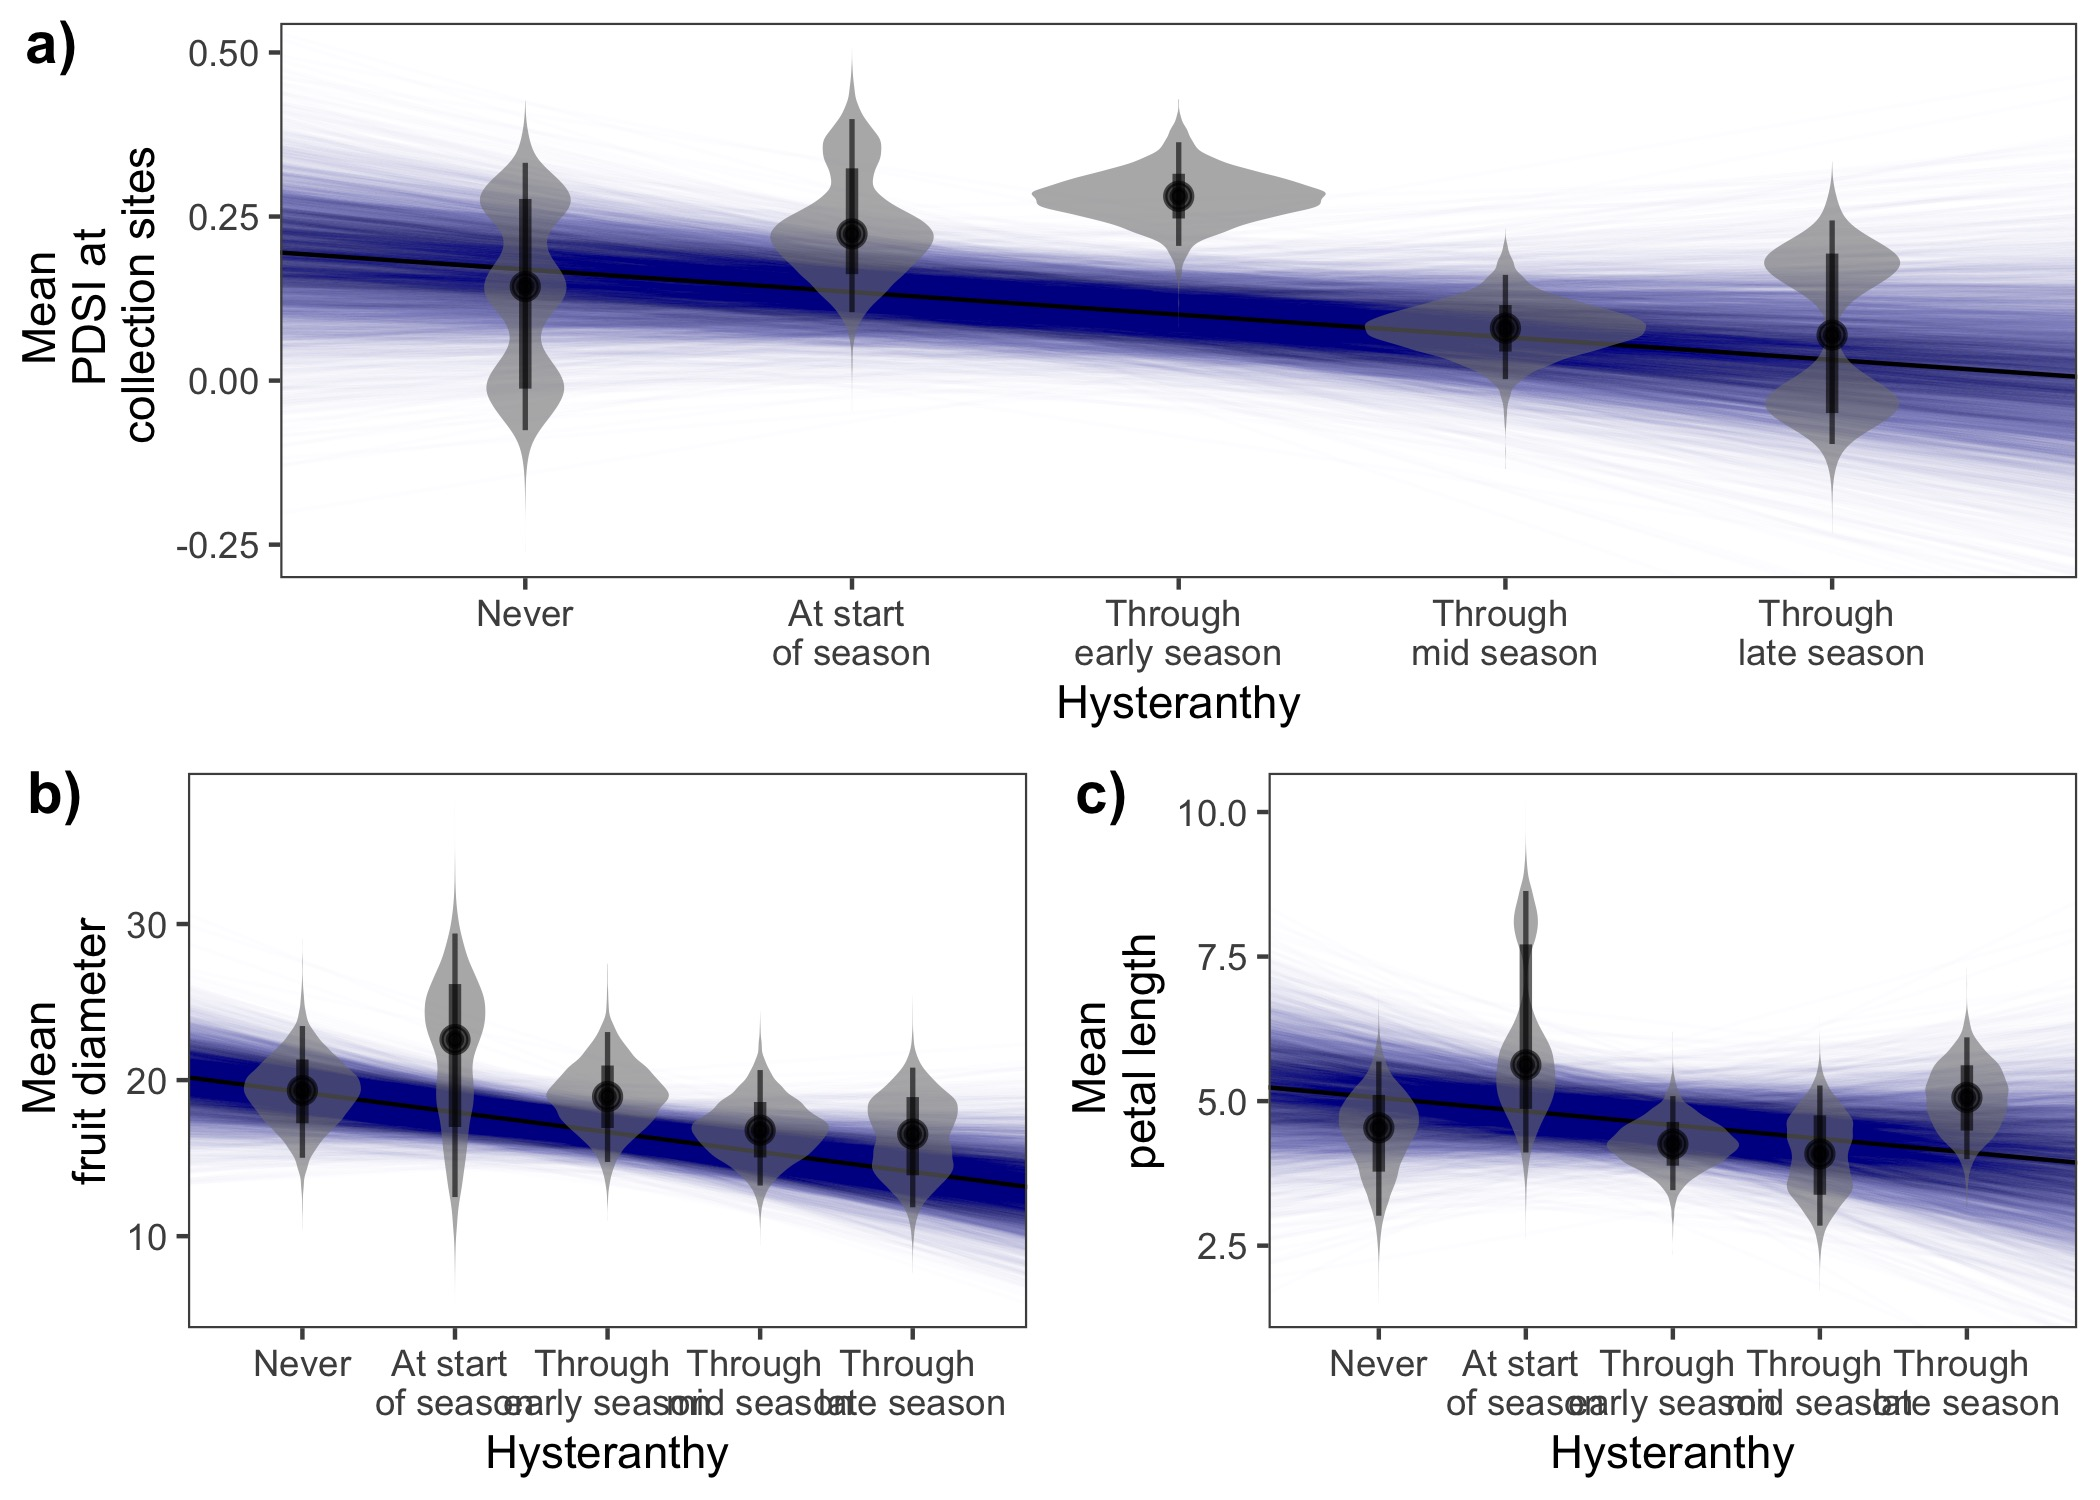
\includegraphics[width=\textwidth]{..//..//Plots/dataplots.jpeg}
    \caption{Relationships between the duration of hysteranthy across the flowering period and environmental and biological traits  }
    \label{fig:prunes}
\end{figure}


%\begin{figure}[h!]
 %   \centering
 %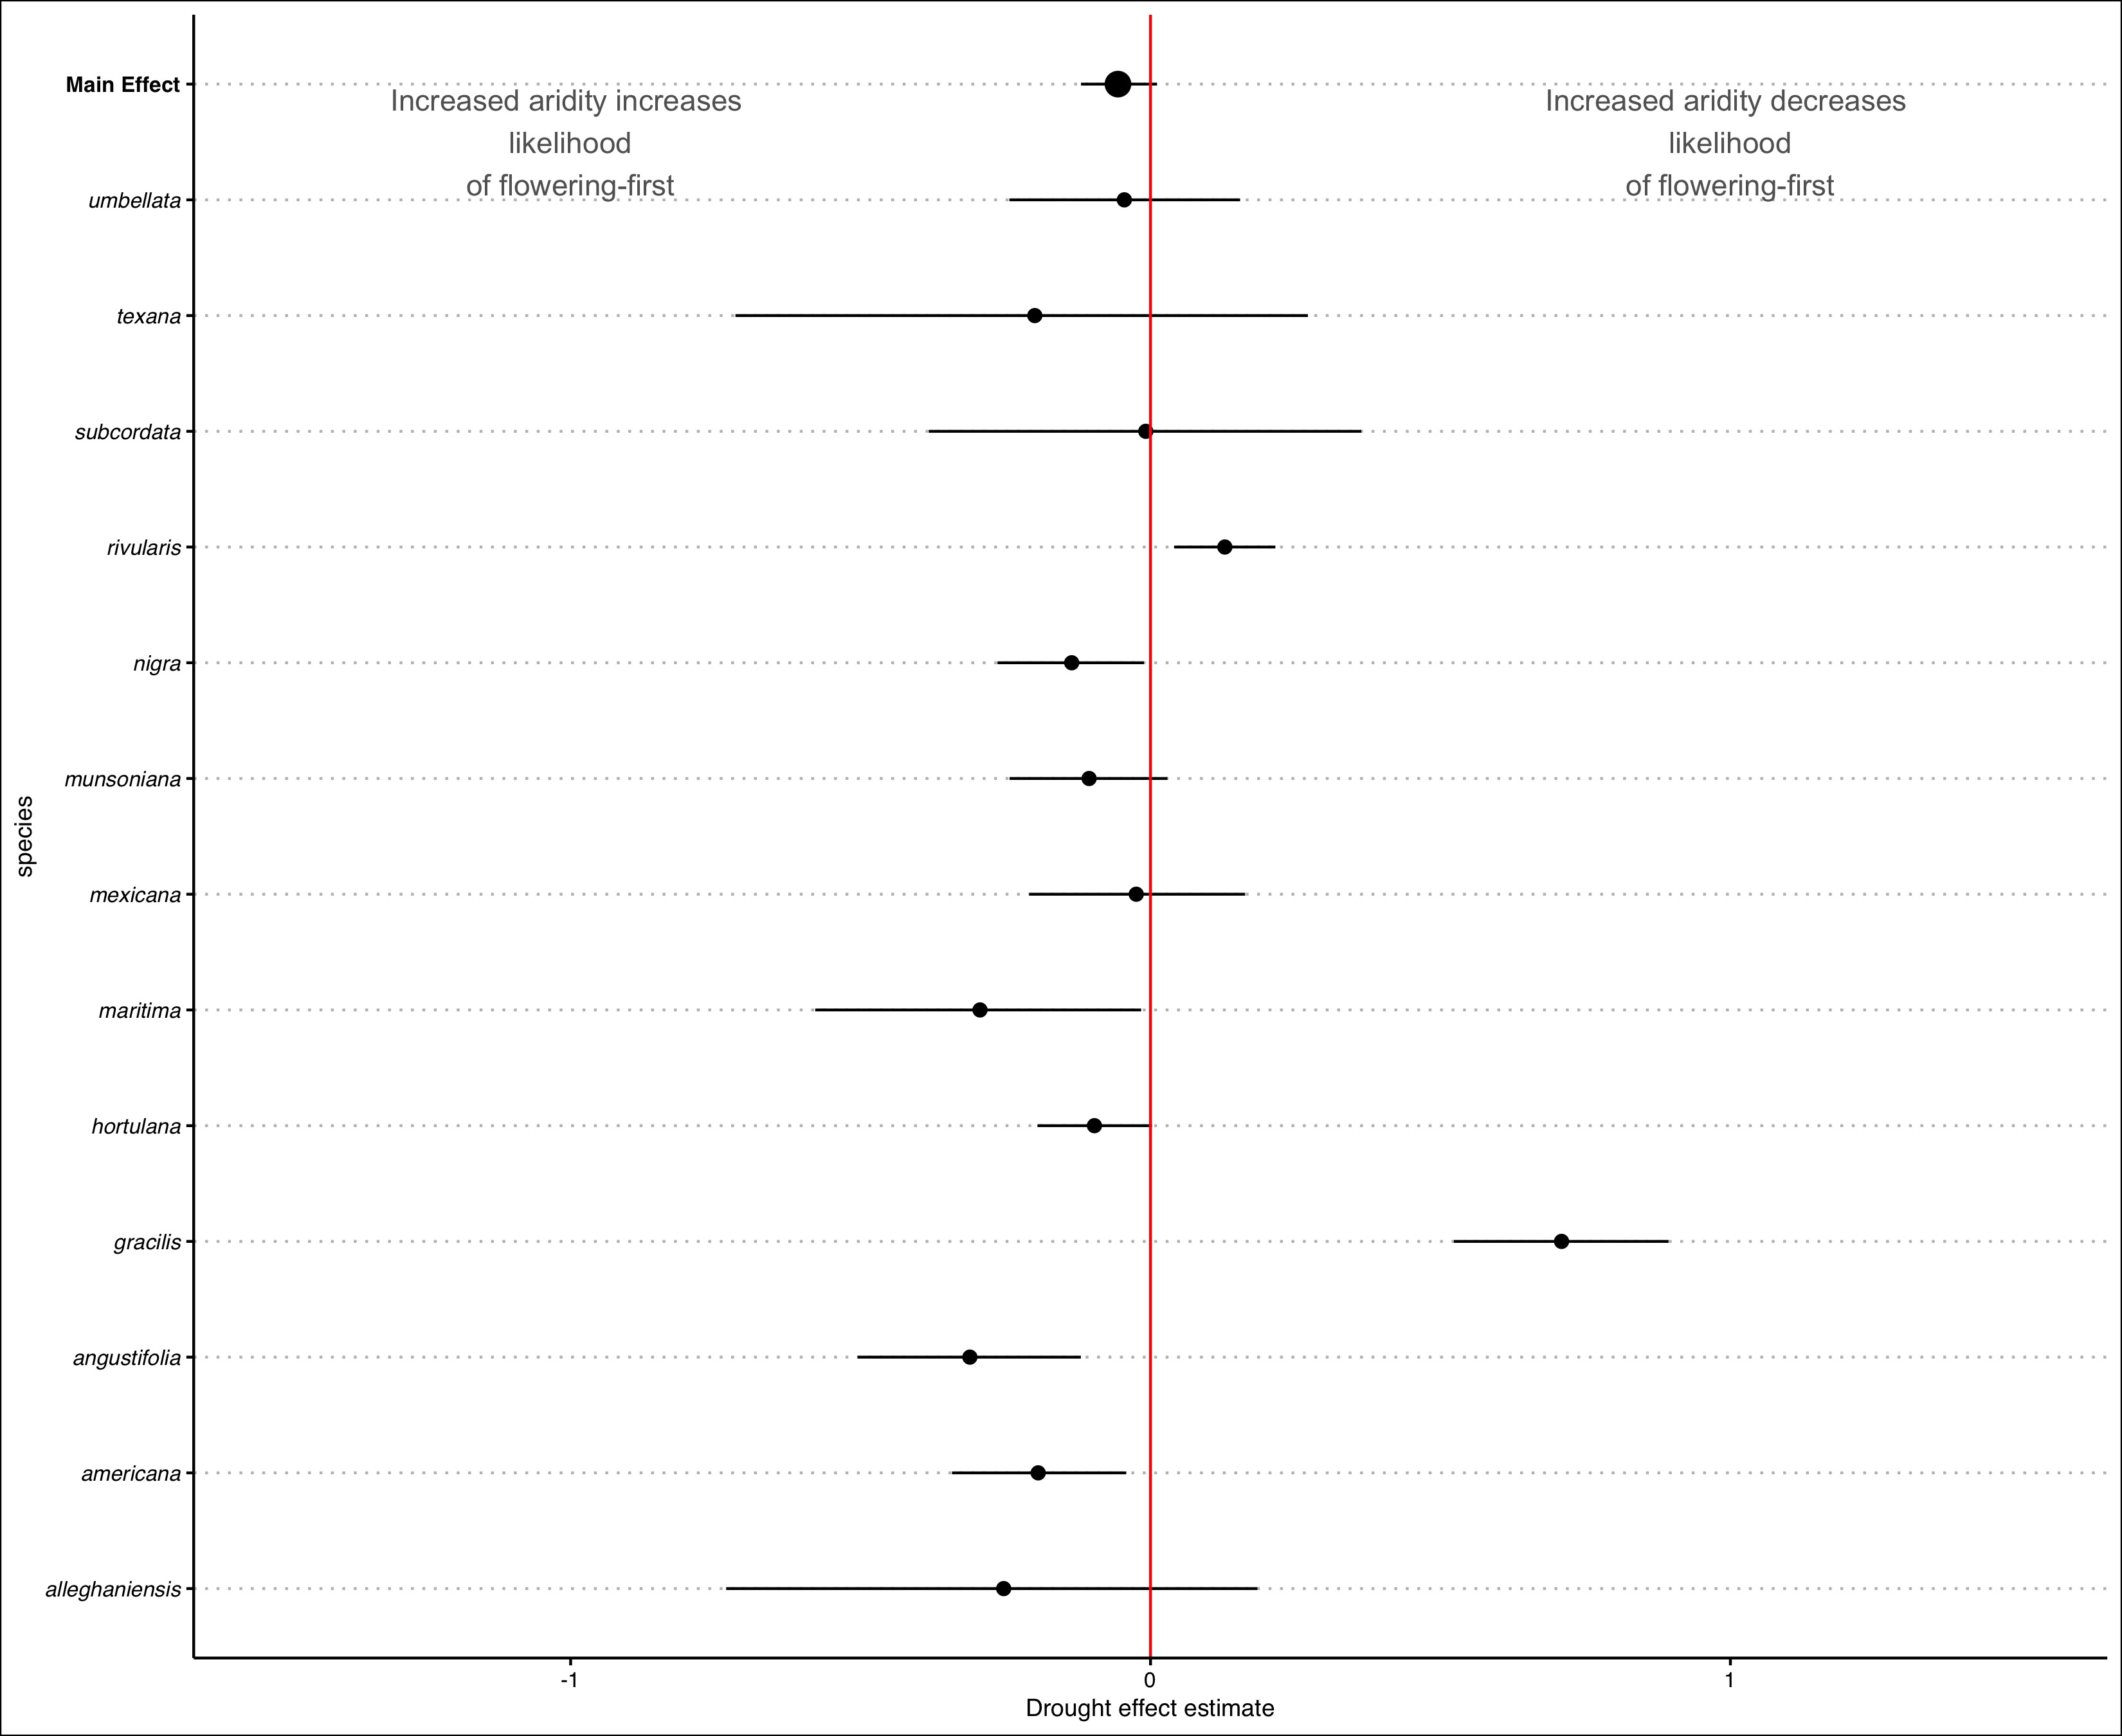
\includegraphics[width=\textwidth]{..//..//Plots/droughtstuff.jpg}
  %  \caption{Hysteranthy more likely in drought years.}
   % \label{fig:plastic}
%\end{figure}

\end{document}
